\chapter{One stage OTA}

\centering
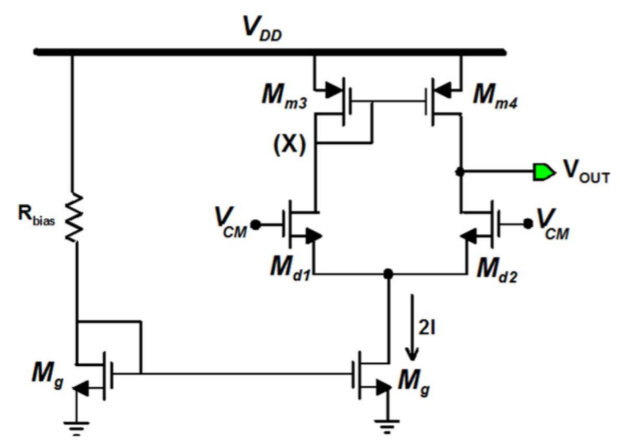
\includegraphics[width=0.5\textwidth]{OTA1.png}\\
\raggedright

\section{Dynamics}

\subsection{n-mos stage}

\begin{wrapfigure}{i}{0pt}
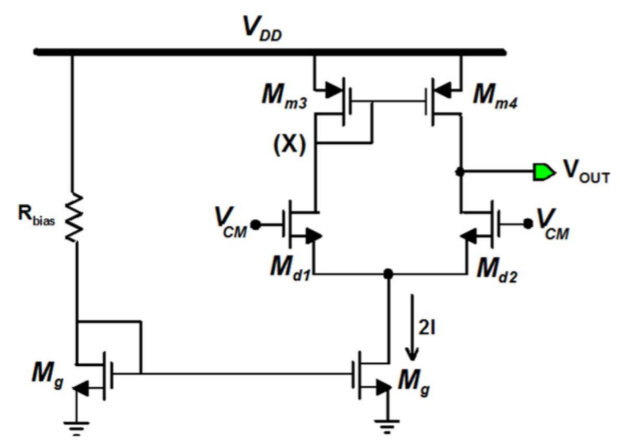
\includegraphics[width=0.25\textwidth]{OTA1.png}
\end{wrapfigure}

Common mode dynamic
\begin{equation}
V_{CM}^{min}=V_{ov}^{mg}+V_{gs}^{in}\ \ \ \ \ \ \ \ \ \ \ \ \ \ \ V_{CM}^{max}=V_{dd}-V_{gs}^{mM}+V_t^{in}
\end{equation}
Output dynamic 
\begin{equation}
V_{out}^{min}=V_{CM}-V_t^{in}\ \ \ \ \ \ \ \ \ \ \ \ \ \ \ V_{out}^{max}=V_{dd}-V_{ov}^{mM}
\end{equation}
\vspace{1mm}

\subsection{p-mos stage}

\centering
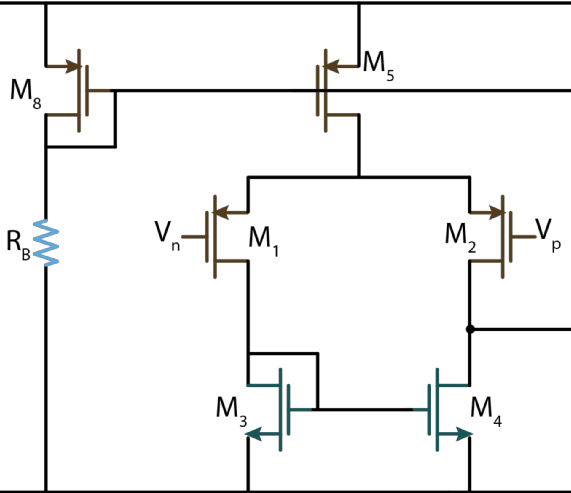
\includegraphics[width=0.35\textwidth]{OTA2.png}\\
\raggedright

Common mode dynamic
\begin{equation}
V_{CM}^{min}=V_{gs}^{m3}-V_t 
\end{equation}
\begin{equation}
V_{CM}^{max}=V_{dd}-V_{OV}^{m5}-V_{sg}^{m1}
\end{equation}

\section{Differential gain}
\begin{equation}
G_d=g_{m1}r_{0,2}//r_{0,4}
\end{equation}

\section{Common mode gain}
\begin{equation}
G_{CM}=\frac{\varepsilon(r_{0,2}//r_{0,4})}{r_{0,g}}
\end{equation}
The variable $\varepsilon$ has 2 dependance on deterministic and non deterministic effects.

\subsection{Deterministic contributions}
{\bf Mirror error}\\
Current read from M3 is a partition ,caused by $r_03$, of the total current.
\begin{equation}
\varepsilon_{det,mirror}=\frac{1/g_{mM}}{1/g_{mM}+r_{03}}=\frac{1}{1+g_{mM}\cdot r_{03}}\simeq \frac{1}{g_{mM}\cdot r_{03}}
\end{equation}
{\bf Unballace of the stage}\\
The impedence seen from the source of the input generators if the two branches is not the same.
\begin{equation}
\varepsilon_{det,unballace}\simeq \frac{1}{r_{01}\cdot g_{mM}}
\end{equation}

\subsection{Statistical contributions}
{\bf Statistical mismatch of the mirror}\\
Taking $\Delta g_{m}=g_{m3}-g_{m4}$ 
\begin{equation}
\varepsilon_{stat,mirror}=\frac{\Delta g_{m}}{g_{m}}
\end{equation}
{\bf Statistical mismatch of the input mos}\\
Taking $\Delta g_{m}=g_{m1}-g_{m2}$ and $g_{m}=(g_{m1}+g_{m2})/2$
\begin{equation}
\varepsilon_{stat,input}=-\frac{\Delta g_{m}}{g_{m}}(1+\frac{2r_{0G}}{r_{01}})
\end{equation}

\section{CMRR}
\begin{equation}
CMRR=G_d/G_{CM}=\frac{2g_{m1}r_{0g}}{\varepsilon}
\end{equation}

\subsection{Deterministic CMRR}
Common mode rejection ratio due to deterministic effect
\begin{equation}
CMRR_{det}\simeq \frac{2g_{m1}r_{0g}}{\frac{1}{g_{mM}\cdot r_{03}}+\frac{1}{r_{01}\cdot g_{mM}}}
\end{equation}

\subsection{Statistical CMRR}
Common mode rejection ratio due to statistical effect with very bit $r_g$ approaches to
\begin{equation}
CMRR=G_d/G_{CM}=\frac{2g_{m1}r_{0g}}{\varepsilon_{stat}}\rightarrow \frac{g_{mM}\cdot r_01}{\frac{\Delta g_{m1}}{g_{m1}}}
\end{equation}

\section{Input voltage offset}
Input voltage offset caused due to statistical unbalace of the transistors.\\
\subsection{Input mismatch}

Offset caused by k variations
\begin{equation}
V_{OS}^{in,k}=\frac{V_{ov1}}{2}\cdot \frac{\Delta k}{k}
\end{equation}

Offset caused by $V_t$ variatons
\begin{equation}
V_{OS}^{in,V_t}=\Delta V_t
\end{equation}

So the total offset due to input transistors is 
\begin{equation}
V_{OS}^{in}=\frac{V_{ov1}}{2}\cdot \frac{\Delta k}{k}+\Delta V_t
\end{equation}

\subsection{Mirror mismatch}

Offset caused by k variations
\begin{equation}
V_{OS}^{mirror,k}=\frac{V_{ov,g}}{2}\cdot\frac{\Delta k_M}{k_M}
\end{equation}

Offset caused by $V_t$ variations 
\begin{equation}
V_{OS}^{mirror,V_t}=\frac{V_{ov,g}}{V_{ov,m}}\Delta V_{t,M}
\end{equation}

\subsection{Total offset}
Defining with the Pelgrom constants the factors
\begin{equation}
\sigma^2(\frac{\Delta k}{k})=\frac{K^2_{\Delta k/k}}{WL}\ \ \ \ \ \ \ \ \ \ \ \ \ \ \sigma^2(\Delta V_t)=\frac{K^2_{\Delta V_t}}{WL}
\end{equation}
we can define the statistic offset as 
\begin{equation}
\sigma(V_{OS})=\sqrt{\sigma^2(\Delta V_{t,in}) +\sigma^2(\Delta V_{t,M})\cdot \left(\frac{V_{ov,in}}{V_{ov,M}}\right)^2+\left(\frac{V_{ov,in}}{2}\right)^2[\sigma^2(\frac{\Delta k}{k}_{in})+\sigma^2(\frac{\Delta k}{k}_M)]}
\end{equation}


\section{Input equivalent noise}

\subsection{White noise}
Voltage noise: 
\begin{equation}
S_v^{in}=\frac{8kT\gamma}{g_{m1}}(1+\frac{g_{mM}}{g_{m1}})=\frac{8kT\gamma}{g_{m1}}(1+\frac{V_{ov,in}}{V_{ov,m}})
\end{equation}
Current noise:
\begin{equation}
S_i^{in}=kT\gamma(4g_{m,in}+2g_{m,M}+g_{m,G})(\frac{\omega}{\omega_T})^2
\end{equation}
With $\omega_T=\frac{1}{C_{gs}1/g_m}$ cut off radial frequency. This noise has a quadratic dependence with frequency.\\
The voltage noise is dominant over the current one until the crossover frequency
\begin{equation}
f\simeq \frac{f_t}{g_mR_s}
\end{equation}
with $R_s$ input resistance of the circuit. In practice we will current noise is considered only in RF applications.

\subsection{Nigger 1/f noise}
Same transfer of the white noise but the current generator is 
\begin{equation}
S_I(f)=\frac{K^{1/f}}{C_{ox}'WL}
\end{equation}
So the overall tranfer function is 
\begin{equation}
E_{1/f}=[\frac{K^{1/f}}{C_{ox}'W_{in}L_{in}}+\frac{K^{1/f}}{C_{ox}'W_{mM}L_{mM}}\left(\frac{g_{m}^{mM}}{g_{m}^{m,in}}\right)]\frac{1}{f}
\end{equation}


